\pdfoutput=1

\documentclass{l4proj}
\usepackage{url}
\usepackage{subcaption}
\usepackage{float}
% compacting the list items
\usepackage{enumitem}
\usepackage{multirow}
\usepackage{booktabs}
\usepackage{tabularx} % in the preamble
\usepackage{adjustbox}

%
% put any packages here
%

\begin{document}
\title{Urban Data Timeline}
\author{Yordan Yordanov}
\date{March 28, 2016}
\maketitle

\begin{abstract}
We show how to produce a level 4 project report using latex and pdflatex using the 
style file l4proj.cls
\end{abstract}

\educationalconsent
%
%NOTE: if you include the educationalconsent (above) and your project is graded an A then
%      it may be entered in the CS Hall of Fame
%
\tableofcontents
%==============================================================================

\chapter{Introduction}
\pagenumbering{arabic}

\section{Motivations}
\paragraph{}
Smart cities bring a lot of advantages. They can opt for better urban planning and development by making more efficient use of the infrastructure to improve productivity and services but also to reduce the waste of fuel and energy. Furthermore their intelligence can change and enhance the way authorities respond to changing circumstances. On the other hand, achieving all these goals is a challenging process. Huge amounts of information, created by social feeds, environmental sensors, traffic, news and many more, have to be gathered, stored and analysed. This project aims to combine and visualise all these data strands so that some can look at the cities from a different angle and possibly extract new tendencies and patterns, not possible to discover by following only a single source. This will help us identify problems or challenges that we had not been aware of and provide effective solutions that we all as citizens can only benefit from.

\section{Aims}
\paragraph{}
This project aims to build a tool for the fusion and visualisation of timely data collected from the UBDC for their project, described earlier (iMCD). Past data from various urban data streams, such as social media posts, news, blogs, traffic information, environmental sensors and many more has been provided. The tool should be able to query all this data and come up with a timeline representation of observations that might be of interest to the user. This application is initially build to be used by the \textbf{general public} but may as all be valuable to local researchers who follow or compare people’s opinions, businessmen who want to know how their business is developing, media that want to report what are the public impressions about an important event and even politicians while running their campaigns.   

\section{Background}
\paragraph{}
Smart cities today represent a perception to integrate both information and communication technologies in an acceptable and maintainable fashion to manage their infrastructure and facilities. The optimal goal is to enhance the quality of life and satisfy the residents’ needs. ICT gives to the people, who maintain these cities, the great opportunity to directly follow what is happening and take actions accordingly. This can be done only by processing the huge amounts of information, collected from sensors, in real time and providing knowledge and information: the keys for discovering inefficiencies. 
\paragraph{}
However, the biggest asset of a smart city is not the number of cameras or sensors but the people that occupy it. A third of the internet users\cite{ofcomreport1} represent their smartphone as the most important device for going online. A third of the population owns a smart device and use it every day to bank, shop and access social media. Social media streams, such as Twitter, have a reputation to be extremely useful source of information. Anybody can understand what is happening all around the world in real time. With that comes various opportunities for developers to implement systems that automatically detect and track events as they happen. Smart cities can benefit from that as what better way to improve efficiency than for example identifying and reporting road accidents to the emergency services in real time.
\paragraph{}
Aiming to help with analyzing these massive amounts of data, the Urban Big Data Centre was established by the UK Economic and Social Research Council to address social, economic and environmental challenges facing cities. Their researchers are undertaking innovative projects, covering topics from big data management to linking and analysing the multi-structural urban data.  Such project is the Integrated Multimedia City Data. 



\subsection{Integrated Multimedia City Data}

\paragraph{}
Integrated Multimedia City Data\cite{imcd} (iMCD) is one of the Urban Big Data Centre’s inaugural projects, funded by the Economic and Social Research Council. It is designed to provide the UBDC with innovative primary data sources. The project consists of four strands: representative household survey, tracking of real-time urban sensors, internet based visual media collection and internet based textual media collection.  
\paragraph{}
The core research strand is the representative household survey that aims to gather data about people’s attitude and behaviour when it comes to information and communication technologies, traveling and learning. Some of the participants are given GPS and life logging sensors that record their activities and travel. Meanwhile the visual and textual data, referring to Glasgow and surrounding areas, is to be collected from the internet. 
\paragraph{}
All of these strands, together, are able to show how Glasgow performs as a smart city.  The Terrier IR team provides various data web services so that all these sources can be browsed and queried.

\subsection{Terrier IR}
\paragraph{}
Tell a bit about Terrier IR

\subsection{Web Services}
\paragraph{}
Describe what a web service is

\subsection{Web Application}
\paragraph{}
Describe what a web application is

\section{Outline}
The rest of the report is structured as follows:
\begin{itemize}
	\item \textbf{Chapter 2} provides an overview of related work with examples of similar applications.
	
	\item \textbf{Chapter 3} discusses the project planning by separating it into project approach and requirements engineering.
	\item \textbf{Chapter 4} explains the design by showing the initial paper prototypes and architectural diagrams. It also provides a comparison between the possible technologies, that are available and suitable for such a project.
	\item \textbf{Chapter 5} goes through the actual implementation of each component and describes the challenges faced. 
	\item \textbf{Chapter 6} describes the two phases of the evaluation process and explains the testing strategy for the components.
	\item \textbf{Chapter 7} concludes the report and discusses the implication of the evaluations in terms of future directions
\end{itemize}


\chapter{Related Work}
\paragraph{}
There are applications that have been developed to accomplish similar if not the same goals. This chapter is presenting a short description of related products, along with key differences and correlations in comparison with the goals of this project.  

\subsubsection{Google Maps Timeline} 
\paragraph{}
Google stores a history of where anybody that uses its location services goes. All this data is collected by your device sensors and the navigation you use. Then it is visualized with the Google Maps Timeline \cite{GoogleMapsTimeline} feature. This application is advertised to be an easy way to view and remember places somebody has been on a given day at a given time. Without any input, the timeline shows predictions of when you have arrived or left a place. One of the key features is highlighting when you have visited the most places and how you had travelled. The application does not offer sharing as Google wants your information to remain private. As far as human interaction goes, you are allowed to correct, confirm or delete a place where Google thinks you had been but even after deleting,  it can still be seen that you had passed by that area. In 2009, the company released a similar feature called Google Latitude that offered sharing of location history but the project was closed down \cite{GMTimeFeature}.

\paragraph{}
This product has the same initial goal to visualize timely data originating from different streams like navigation history, pictures, travel and walking routes. Some of the key features are using a vertical timeline to display the events, allowing searching based on a specific day, month, year and having a way to show (via bar chart) how active you have been every day in the past few weeks. 

\subsubsection{Social Media Timeline}
\paragraph{}
All social media websites in the likes of Twitter and Facebook use some sort of a timeline to visualize their user's personal information. However they differ on the way they organize their posts. Facebook describes a timeline to be a place on your profile where you can see your own posts, your friends' activities and stories you're tagged in, sorted by the date and time they were posted. On the other hand, Twitter displays a stream of tweets from accounts that you have chosen to follow. Making use of machine learning algorithms, posts that you are likely to care about more are displayed first.
\paragraph{}
Despite the fact that social media applications have as a main goal the delivery of a secure and reliable tool for communication, they also provide their users with the ability to visualize their personal data streams like photos, events, group activities and accomplishments. Both Facebook and Twitter use a vertical timeline and allow for searching based on keywords. One of the key features is infinite scrolling that make the illusion of one endless stream of events by making use of the million users, posting every day. 

\subsubsection{Tech City Map}
\paragraph{}
Tech City Map pulls streams of social media posts for all the businesses in the East London area and tries to analyse their influence. The idea lies on using a map to display all the corporations in the area and linking them together by using different coloured lines for any tweet from one business to the other. The tool allows searching for a specific company as some points represents more then one corporation and manually searching though the map can be difficult. From 2010 to 2012\footnote{http://flowingcity.com/visualization/tech-city-map/} the number of businesses in East London had risen from 200 to 600. This growth was welcomed even by the Prime Minister at that time, David Cameron, proving that such tools are even followed by politicians. 

\subsubsection{Conclusion}
\paragraph{}
Some of the previously described applications are proven to be successful by millions of users all around the world. However, they focus only on their user and do not really visualise and offer a big variety of data sources. On the other hand, Urban Data Timeline targets the smart city by increasing the user's understating about it. Furthermore, with the help of the Urban Big Data Centre, it has plenty data streams to offer: querying a tweet collection based on a hashtag or specific tweet terms, examining the events, detected by automated systems, related to specific terms, obtaining information about busy venues in an area of a city, finding train stations within a radius of a specific location, searching for delayed trains and accessing past weather data records. Also, all these big companies like Google, Facebook and Twitter provide their own APIs. This brings a great opportunity for this innovative project to become a centralised system where, for example, busy venues can be listed with the tweets from their own Twitter or Facebook accounts and events can be reviewed in depth with the help of news and youtube videos.


\chapter{Project Planning}

\section{Software design approach}
\paragraph{}
When a new product is developed, it is not clear how it will end up and if it will fulfil the user's requirements. The developers can see the first steps but there are plenty of problems or challenges that can not be predicted from the beginning (Figure \ref{projectInitial}). That is true for any project, no matter how much planning is put in. However there is a possibility that everything is done the right way but there is a high probability to drift away from the initial target (Figure \ref{projectStart}). There are several methodologies that can be followed when developing a software but the two most common are Waterfall and Agile. 

\subsection{Waterfall model}
\paragraph{}
The Waterfall model is an example of a plan-driven process - in principle you must plan and schedule all of the process activities before starting work on them \cite{sene}. Here iterations can be costly and involve significant rework. Therefore, after a small number of iterations, it is normal to freeze parts of the development, such as the specification, and continue with the later development stages. Problems are left for later resolution, programmed around or completely ignored. These implementation tricks may also lead to design problems and badly structured systems.

\subsection{Agile model}
\paragraph{}
This project, on the other hand, follows the Agile methodology (Figure \ref{projectAgile}) for software development. It is an interactive
approach that splits the work into a number of iterations (sprints). This allow the project supervisors to inspect the work of the developer and monitor how well the software development is progressing \cite{sene}. Each of these sprints last one
week. It starts with a meeting and demonstration of the work done in the previous sprint. As an
outcome of these meetings feedback from the supervisors is received, based on the
extent to which their requirements are met. Moreover, these meetings allow discussions of the issues
that are experienced and compare the available workarounds. At the end of a meeting, it is agreed
upon exactly what work will be done during the next sprint. Following this scenario, at least one new
feature is introduced after each sprint and changes to previous features are performed as early as possible. By the end of this project, 23 iterations are to be performed.

\begin{figure}[H]
\begin{subfigure}{.3\textwidth}
	\centering
	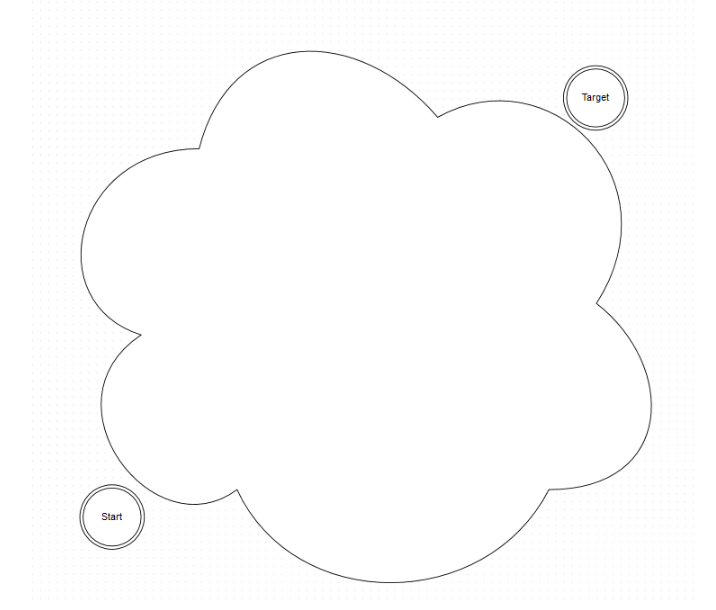
\includegraphics[height=4cm,width=4cm]{images/projectInitial}
	\caption{Start of a project.}
	\label{projectInitial}
\end{subfigure}
\begin{subfigure}{.3\textwidth}
	\centering
	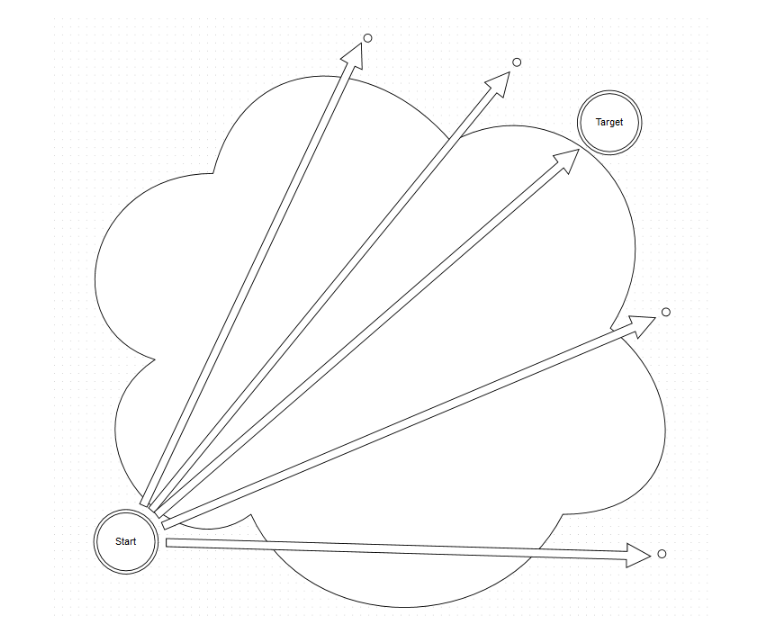
\includegraphics[height=4cm,width=4cm]{images/projectStart}
	\caption{Waterfall methodology.}
	\label{projectStart}
\end{subfigure}
\begin{subfigure}{.3\textwidth}
	\centering
	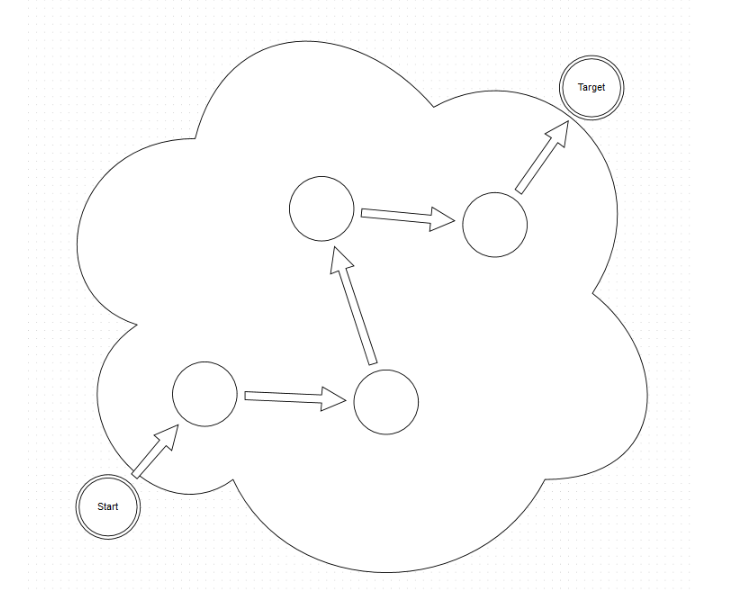
\includegraphics[height=4cm,width=4cm]{images/projectAgile}
	\caption{Agile methodology.}
	\label{projectAgile}
\end{subfigure}
\caption{Software development methodologies}
\end{figure}



\section{Requirements Engineering}
\paragraph{}
The requirements for a system describes the functionality of the services it provides and the constraints of its operation. The process of gathering, analysing and documenting these services and constraints is called requirements engineering.
\paragraph{}
At the beginning of the project, a few weeks were taken to envision the high-level requirements and to understand the scope of the required system. For the initial requirements use cases and user stories were extracted to help with exploring how users will work with the system. 

\subsection{Use cases} 
\paragraph{}
Use case is a way to describe how a real user interacts with the system. They should not be perfect and can only show the action and not go into much detail, in order to stay close to the agile methodology. The developer will implement the system but will have to work close with the supervisors so that the end product will meet their needs. 

The following use cases were identified in the beginning of this project: 


\begin{itemize}%[noitemsep]
	\item see how tweets about a specific hashtag are distributed over a period of time
	\item see popular hashtags that are twitted together with a specific hashtag
	\item get information about a certain area of the city and find out if the venues(restaurants, train stations, cinemas) there get high attendance
	\item browse tweets based on time and hashtag
	\item use the system on a mobile device
	\item check out what the clients post about a venue, they had visited
	\item check how many people attend specific venues in a given area
	\item compare people's opinions about an event
	\item see if a political party is likely to win the elections
\end{itemize}


\subsection{Functional requirements} 
\label{sec:functional-requirements}
\paragraph{}
Functional requirements represent services the system should provide, how it should react to particular inputs and how the system should behave in some situations. More specific requirements can describe the system functions, its inputs and output or exceptions in detail \cite{sene}. 
\paragraph{}
Adding new requirements may change the project direction. Projects usually have fixed duration so sometimes it may not be possible to include all the features. Therefore all use cases that are identified in this chapter must be prioritised. 

\begin{figure}[H]
	\centering
	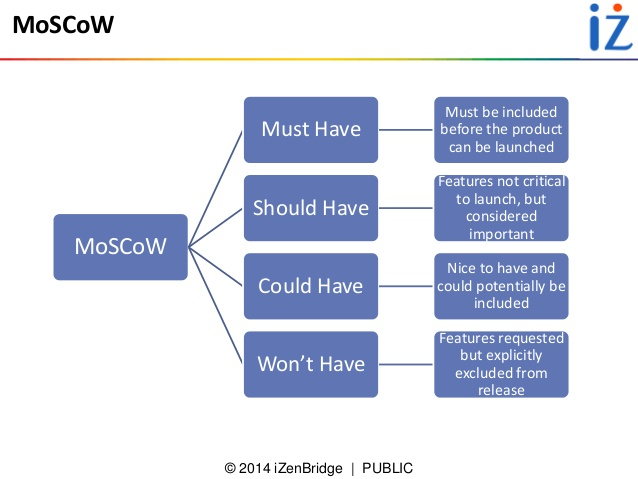
\includegraphics[height=4cm,width=6cm]{images/MoSCoW}
	\caption{MoSCoW rules prioritisation scheme for requirements}
	\label{MoSCoW}
\end{figure} 
\paragraph{}
Figure \ref{MoSCoW} shows the MoSCoW rules that are typically used as a guideline for prioritising requirements. All the use cases should be sorted, using these rules. The ones that are "Must Have" and "Should Have" should be feasible in the duration of the project. Table \ref{tab:funcReq} represents the extracted requirements after their prioritisation. It has now been modified according to the final list of requirements.

%\textbf{\textit{Functional Requirements}}.
%\begin{itemize}
%	\item \textit{User Interface}
%	\begin{itemize}
%		\item Must be able to display a fusion of different kinds of timely data (tweets, weather, traffic, train delays etc.).
%		\item Must be able to show specific as well as general information based on the request.
%		\item Must display events in a timeline.
%		\item Must display the time of events.
%		\item Must be able to take date input.
%		\item Must be able to receive hashtag input.
%		\item Must be able to take location based input.
%		\item Must be able to show venues in specific area. (using a Map)
%		\item Should dynamically add data to the layout. (using AJAX)
%		\item Should be able to visualise statistic data on a graph.
%		\item Could show a summary of the made request.
%		\item Could show the link of an event with other events.
%	\end{itemize}
%	
%	\item \textit{Server}
%	\begin{itemize}
%		\item Must be able to fetch data from provided services.
%		\item Must be able to fetch data from external sources. (Twitter)
%		\item Should provide additional RESTful APIs. (TODO: explain what is REST)
%		\item Should support caching.
%		\item Could store pre-render events. 
%		
%	\end{itemize}
%\end{itemize}   

\begin{table}[ht]
	\centering
	\begin{adjustbox}{width=1\textwidth}
		\begin{tabular}{|c|@{}c@{}|}\hline
			\multicolumn{2}{|l|}{\textbf{Functional Requirements}} \\\hline
			\textbf{MoSCoW} & \textbf{User Interface} \\ \hline
			Must
			&
			\begin{tabularx}{\textwidth}{l}
				be able to display a fusion of different kinds of timely data (tweets, weather, traffic, train delays etc.). \\\hline
				be able to show specific as well as general information based on the request. \\\hline
				display events in a timeline. \\\hline
				display the time of events. \\\hline
				be able to take date input. \\\hline
				be able to receive word based input. \\\hline
				be able to take location based input. \\\hline
				be able to show venues in specific area. (using a Map) \\\hline
				be able to show two events, side by side, so that they can be compared. \\
			\end{tabularx}
			\tabularnewline\hline
			Should
			&
			\begin{tabularx}{\textwidth}{l}
				dynamically add data to the layout. (using AJAX) \\\hline
				be able to visualise statistic data on a graph. \\
			\end{tabularx}
			\tabularnewline\hline
			Could
			&
			\begin{tabularx}{\textwidth}{l}
				show a summary of the made request.	\\\hline
				show the link of an event with other events.\\
			\end{tabularx}
			\tabularnewline\hline
			
			& \textbf{Server} \\ \hline
			Must
			&
			\begin{tabularx}{\textwidth}{l}
				be able to fetch data from provided services. \\\hline
				be able to fetch data from external sources. (Twitter) \\
			\end{tabularx}
			\tabularnewline\hline
			Should
			&
			\begin{tabularx}{\textwidth}{l}
				provide additional RESTful APIs. (TODO: explain what is REST) \\\hline
				support caching. \\
			\end{tabularx}
			\tabularnewline\hline
			Could
			&
			\begin{tabularx}{\textwidth}{l}
				store pre-render events. \\
			\end{tabularx}
			\tabularnewline\hline
			
		\end{tabular}
	\end{adjustbox}
	\caption{Functional Requirements}
	\label{tab:funcReq}
\end{table}


\subsection{Non-Functional requirements}
\paragraph{}
Non-functional requirements represent constraints on the services or functions offered by the system. They often apply to the application as a whole, rather than individual components \cite{sene}. Table \ref{tab:nonFuncReq} represents the extracted non-functional requirements for this project. 

%	\textbf{\textit{Non-Functional Requirements}}.
%	\begin{itemize}
%		\item Must be universal to support all kinds of users(citizen, scientist, researchers, local authorities)
%		\item Must be extensible so that different things can be rendered on the views.
%		\item Must be able to quickly process the data from the services.
%		\item Should be accessible from and compatible with desktops, laptops, tablets and smartphone devices.
%		\item Should be testable.
%		\item Should be scalable so that new services can be added.
%		\item Could be compatible with tools that can measure code quality. (Sonar)
%	\end{itemize}

\begin{table}[ht]
	\centering
	\begin{adjustbox}{width=1\textwidth}
		\begin{tabular}{|c|@{}c@{}|}\hline
			\multicolumn{2}{|l|}{\textbf{Non-Functional requirements}} \\\hline
			\textbf{MoSCoW} & \textbf{Requirement} \\ \hline
			Must
			&
			\begin{tabularx}{\textwidth}{l}
				be universal to support all kinds of users(citizen, scientist, researchers, local authorities). \\\hline
				be extensible so that different things can be rendered on the views. \\\hline
				be able to quickly process the data from the services. \\
			\end{tabularx}
			\tabularnewline\hline
			Should
			&
			\begin{tabularx}{\textwidth}{l}
				be accessible from and compatible with desktops, laptops, tablets and smartphone devices. \\\hline
				be testable. \\\hline
				be scalable so that new services can be added. \\
			\end{tabularx}
			\tabularnewline\hline
			Could
			&
			\begin{tabularx}{\textwidth}{l}
				be compatible with tools that can measure code quality. (Sonar) \\
			\end{tabularx}
			\tabularnewline\hline
		\end{tabular}
	\end{adjustbox}
	\caption{Non-Functional Requirements}
	\label{tab:nonFuncReq}
\end{table}
	
\subsection{High Level System Diagram}
\label{sec:highLevelDiagram}
\paragraph{}
The outlined requirements and use cases start to reveal what the system architecture is going to be. In order to achieve the goals, the application has to consist of three main components (Figure: \ref{highLevelDiagram}): client to	handle the	interaction with the user, middleware to handle the application logic, and a database, in our case external services, to store the data. This architectural model is also called Three Tier Architecture. Tiers enable separation of concerns and encapsulate complexity as they can be broken down into layers and sub-tiers. Furthermore, they can be distributed across a number of machines to provide flexibility and can be replicated across a number of machines to provide the really important scalability factor\cite{threetier}.   	

\begin{figure}[H]
		\centering
		\includegraphics[width=.7\linewidth]{images/HighLevelDiagram}
		\caption{High level architecture diagram based on requirements and use cases.}
		\label{highLevelDiagram}
\end{figure}

\subsection{Challenges}
\paragraph{}
After summarising the requirements(Section: \ref{sec:functional-requirements}) and the high level diagram(Section: \ref{sec:highLevelDiagram}), some challenges can be identified. The biggest on is building a system that can be used by people without any experience in computing like citizens and satisfies the needs of researchers. Furthermore, the system should be valuable and usable on mobile devices. Taking into account how many services are to be used, the user interface must be designed carefully and efficiently. Additionally, the services are not implemented specifically for these application so a lot of unrelated data has to be filtered out. Moreover, there are multiple services and all the data, received from them, has to be sorted quickly.   

\subsection{User Stories}
\paragraph{}
User stories are one of the primary development artefacts for Agile project teams. A user story is a high-level definition of a requirement, containing just enough information so that the developer can get a feel of what the user wants to achieve when using the system and performing a task. It represents a functionality that will be of a value to the user. A suggested template for a user story is: 

\begin{center}
	As a \textbf{\textit{ROLE}}, I want to \textbf{\textit{ACTION}}, so that \textbf{\textit{GOAL}}. \cite{sets}
\end{center}
\paragraph{}
The role represents the user that interacts with the system. The action shows how the user wants to use the system and the goal- what the user is trying to accomplish. All user stories are written in a way that they are understandable by both developer and customer. Ideally the customer should write the user stories while discussing them with the developer \cite{sets}. The following list represents the user stories, captured for this project based on the identified target users(TODO: should I talk about target users):    

\begin{itemize}%[noitemsep]
	\item \textbf{\textit{Researcher}}.
	\begin{itemize}
		\item As a Researcher, I would like to see how the tweets for certain query are distributed though out a period of time, so that I can see the pick of the number of tweets.
		\item As a Researcher, I would like to know other popular twitter hashtags for a certain day, so that I can see what was interesting for the Twitter users for that day.
		\item As a Researcher, I would like to know if specific area of the city was busy on a specific date, so that I can see if specific event or weather conditions had affected that area.
		\item As a Researcher, I would like to see a timeline representation of the tweets for a specific query, so that I can follow and see if the user’s opinions change.
		\item As a Researcher, I would like to use the app on a mobile device, so that when I travel, I can continue working on my research.
		\item As a Researcher, I would like to know what were the weather conditions on a specific date and see traffic information, so that I can use the data as an experiment and measure the likelihood of using the public transport when the weather conditions are bad. 
	\end{itemize}
	
	\item \textbf{\textit{Business owner}}.
	\begin{itemize}
		\item As a Restaurant owner, I would like to see if posting a tweet on my timeline affects the number of people that attend my restaurant.
		\item As a Restaurant owner, I would like to see other venues in my area, so that I can check their attendance and try to improve mine.
		\item As a TV channel owner, I would like to compare how many people are talking about my channel at specific time, compared to other channels so that I can change my TV guide and increase my audience.
	\end{itemize}
	
	\item \textbf{\textit{Politician}}.
	\begin{itemize}
		\item As a politician, I would like to compare how popular is my party in the social media in comparison to other parties, so that I can change my campaign and increase my chances of winning.
	\end{itemize}
	
	\item \textbf{\textit{Citizen}}.
	\begin{itemize}
		\item As a citizen, I would like to compare two different public opinions about a specific event, so that I can make a decision of my own. 
	\end{itemize}
\end{itemize}

\chapter{Design}

%\chapter{Solution}
\section{Paper prototypes}
\label{sec:paper-prototypes}
\paragraph{}
As shown on the Figure \ref{uiPrototyping}, designing an interface prototype is an iterative process that consists of four steps. The fist step is determining the needs of the users. This is already discussed in the previous chapter. The second step is building the actual prototype. It is good to start from sketches. One the sketch (Figure: \ref{initialPaperPrototype}) was finished, a wireframe (Figure: \ref{initialWireframe}) was prepared to be evaluated during the next meeting so that changes can be made before the start of the implementation. 

\paragraph{}
During the implementation process, there had been a few changes to the design. In iteration 6, 8(reference progress reports) and 9 new requirements were identified and modifications to the whole design were required (Figures: \ref{finalPrototypeEvent} and \ref{finalPrototypeCompare}). 


\begin{figure}[H]
	\begin{subfigure}{.3\textwidth}
		\centering
		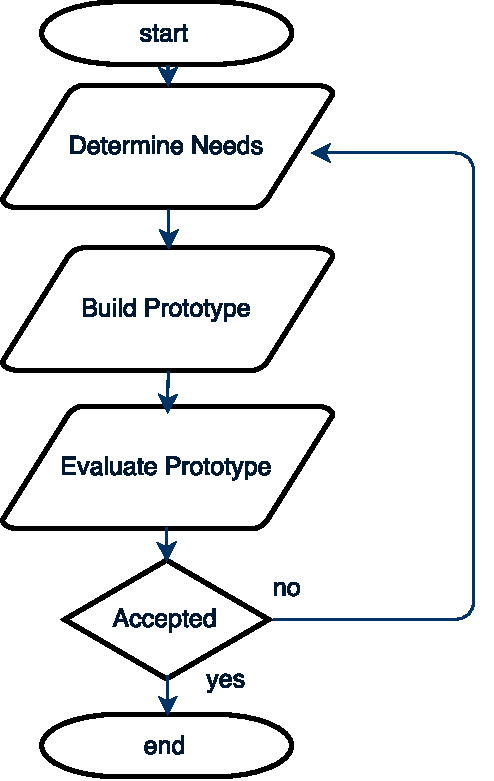
\includegraphics[height=4cm,width=3cm]{images/uiPrototyping}
		\caption{Prototyping process}
		\label{uiPrototyping}
	\end{subfigure}
	\begin{subfigure}{.3\textwidth}
		\centering
		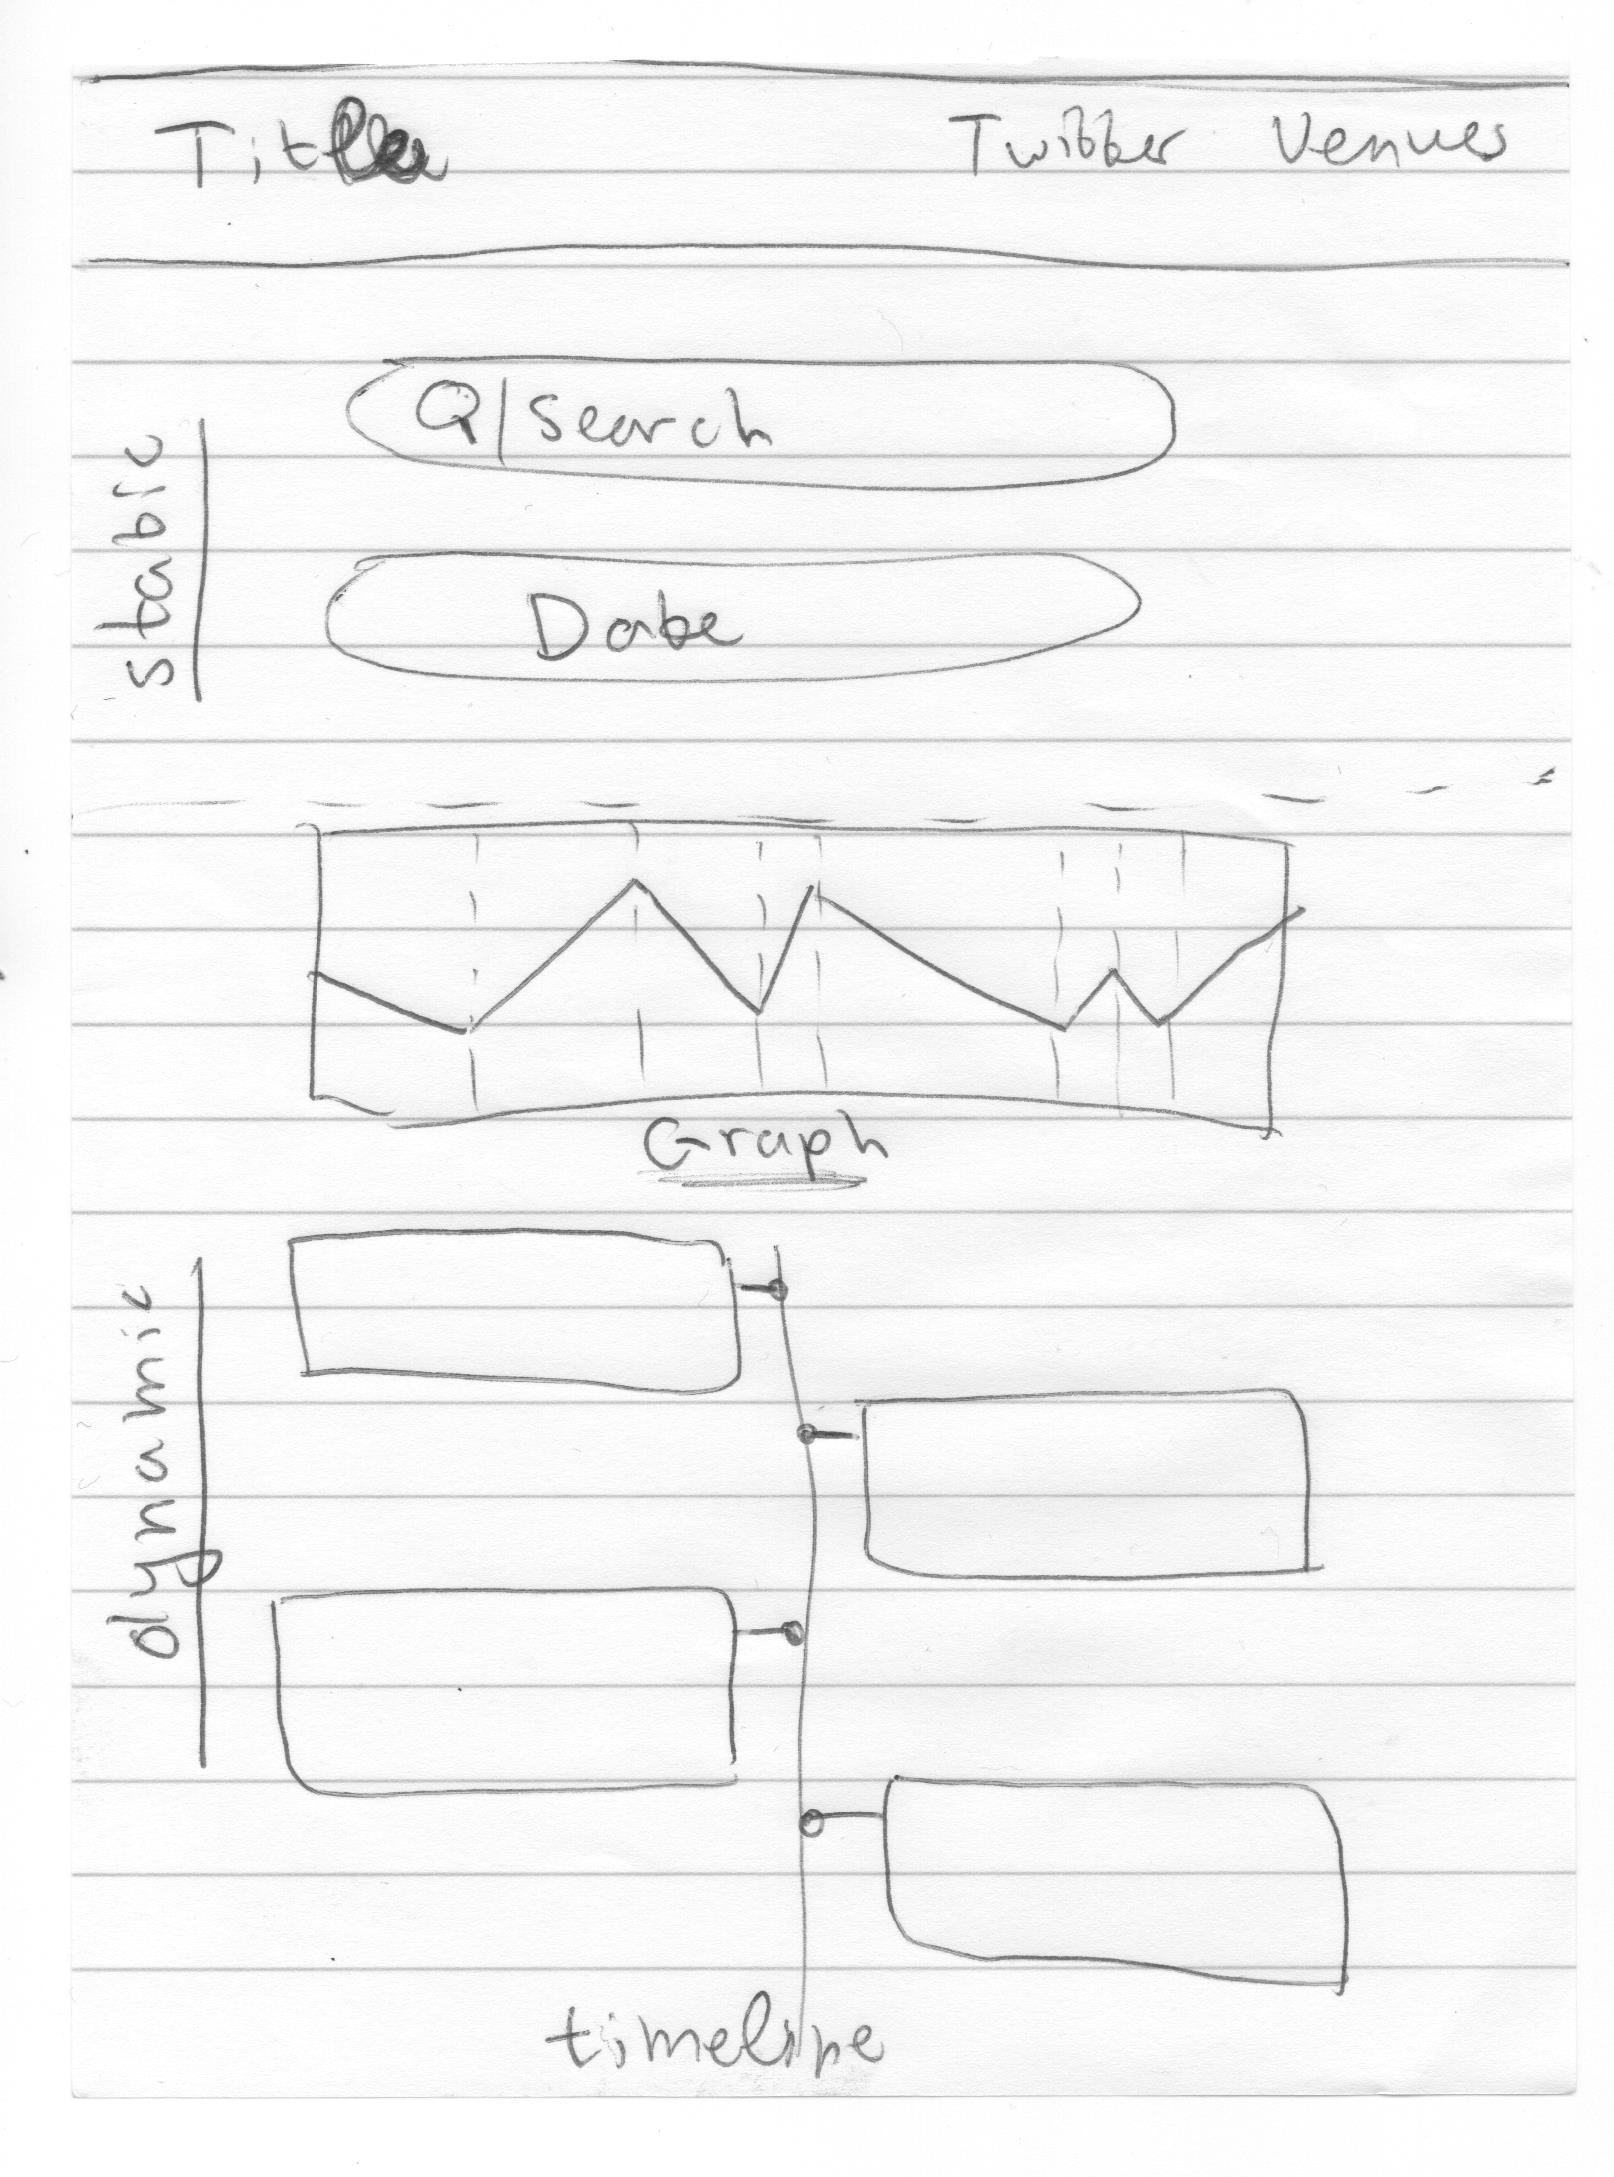
\includegraphics[height=4cm,width=4cm]{images/initialPaperPrototype}
		\caption{Initial Paper Prototype.}
		\label{initialPaperPrototype}
	\end{subfigure}
	\begin{subfigure}{.3\textwidth}
		\centering
		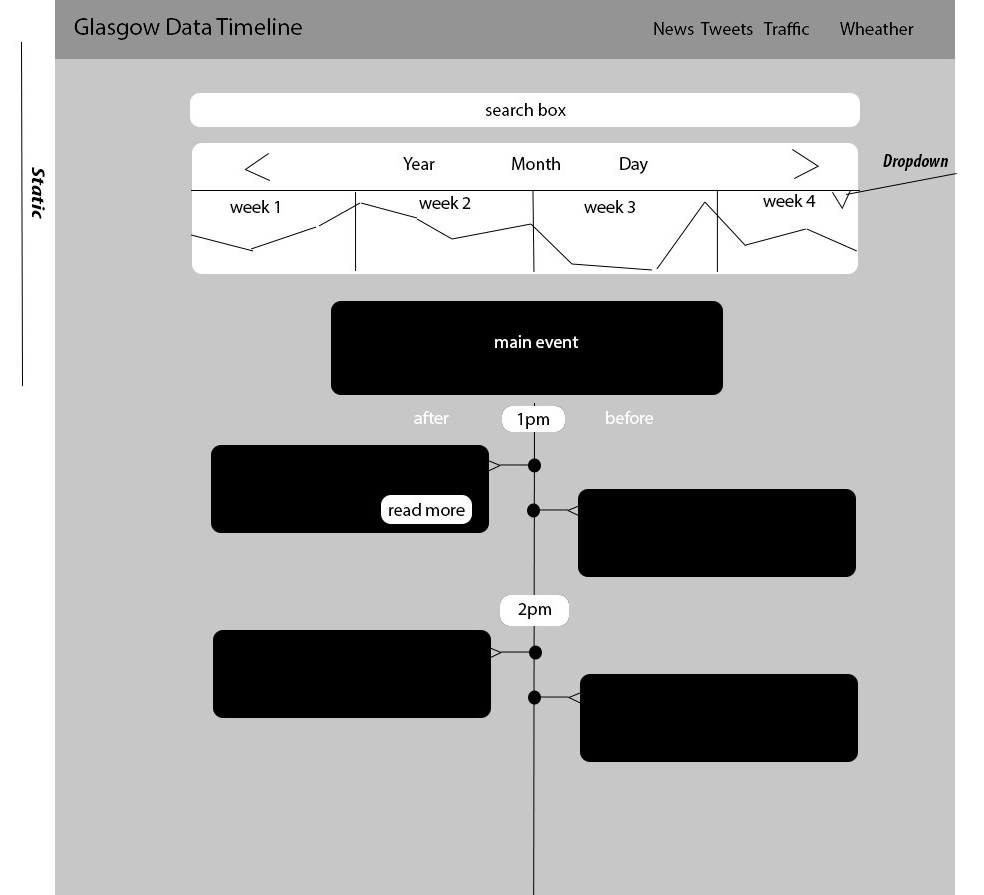
\includegraphics[height=4cm,width=4cm]{images/initialWireframe}
		\caption{Wireframe from the paper prototype}
		\label{initialWireframe}
	\end{subfigure}
	\begin{subfigure}{.3\textwidth}
		\centering
		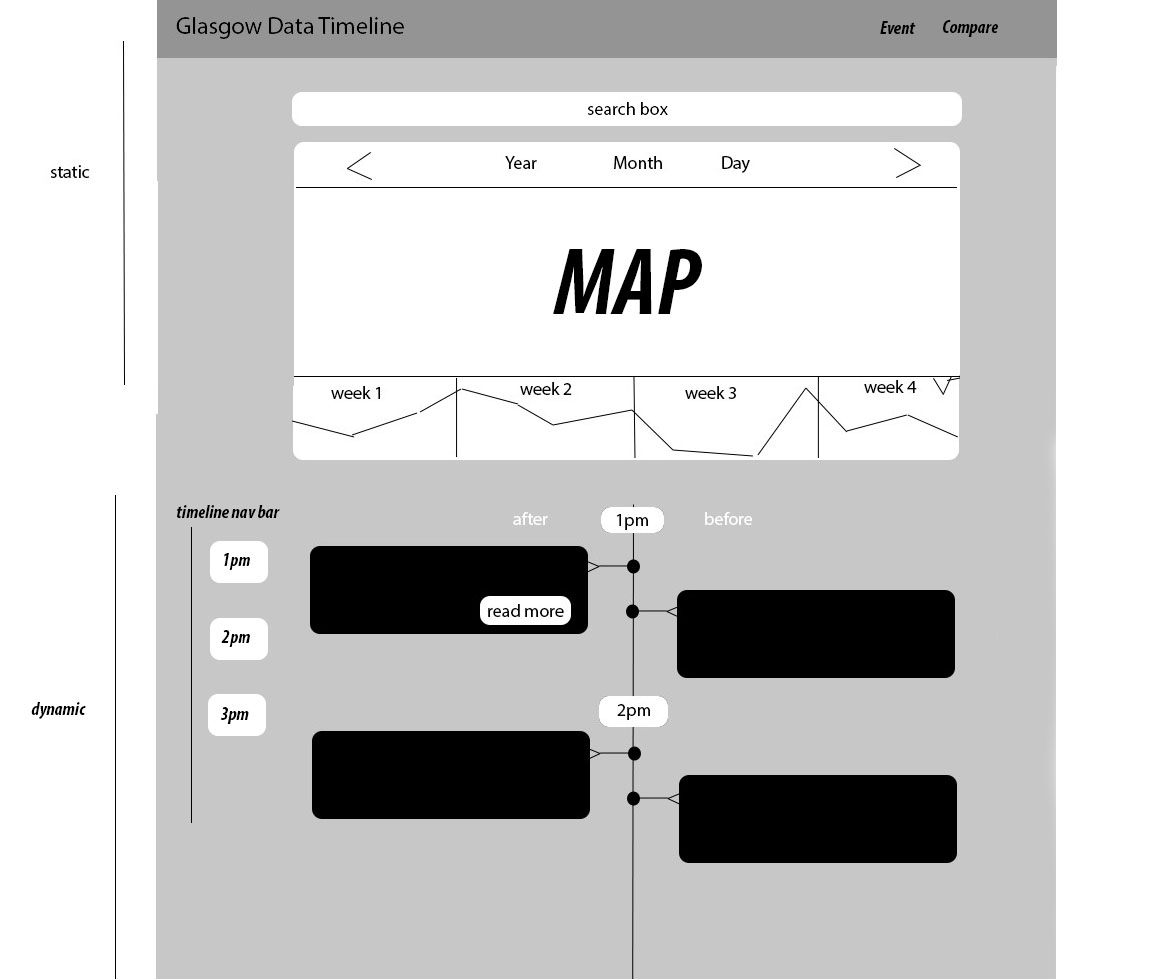
\includegraphics[height=4cm,width=4cm]{images/FinalPrototypeEvent}
		\caption{Wireframe for event exploring}
		\label{finalPrototypeEvent}
	\end{subfigure}
	\begin{subfigure}{.3\textwidth}
		\centering
		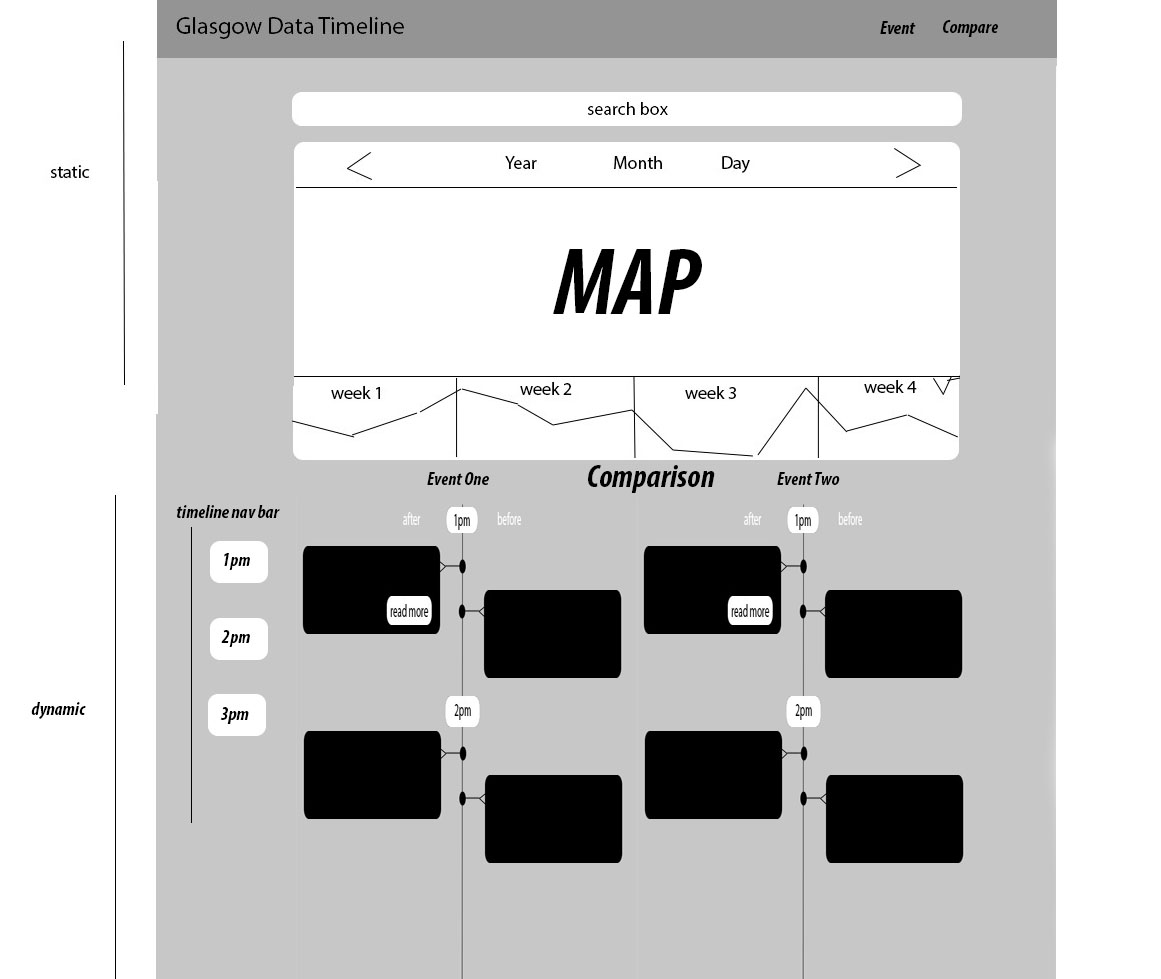
\includegraphics[height=4cm,width=4cm]{images/FinalPrototypeCompare}
		\caption{Wireframe for comparing events}
		\label{finalPrototypeCompare}
	\end{subfigure}
	\caption{Paper Prototypes and Wireframes}
\end{figure} 

\section{Architecture diagrams}
\paragraph{}
The Urban Data Timeline makes use of the Three Tier Architectural model as described in Section \ref{sec:highLevelDiagram}. Based on the diagram, provided in the referenced section, a more in-depth diagram was designed to outline some of the key components of the system (Figure: \ref{componentDiagram}).

\subsubsection{Client}
\paragraph{}
The Client consists of the users and either a mobile device or a desktop PC. The users are going to access the application from the browser, running on their device. The browser talks to both the Google Charts API and Google Maps API, so that it can render the map and the chart, that appear in the wireframes(Figures: \ref{finalPrototypeEvent} and \ref{finalPrototypeCompare}). On the other hand, it talks to the Middleware, or in this case, the Controller component in order to get the information,  required by the user.

\subsubsection{Middleware}
\paragraph{}
The Middleware consists of four components - Controller, View, Cache, and Model. The Controller talks to all of the other components. First of all, the required data is obtained by either the Cache or the Model. If the data is not in the Cache, the Model tries to get it from the external sources. If the communication was successful, the data is stored in the Cache and returned to the Controller. From there, the Controller sends that data to the View so that the page can be prepared and returned to the user. 

\subsubsection{Data}
\paragraph{}
The Data currently consists of two services. The first one is the UBDC web service and it is key to this project as it separates into Twitter, Busy Venue, Delayed Transport, Train and Weather services. As for now, only the first four services are used. The second on is the Twitter API. It is used to compensate for some of the limitations of the other Twitter service, provided by the UBDC, and to broaden the possibilities of tweets querying.        
  

\begin{figure}[H]
	\centering
	\includegraphics[width=\linewidth]{images/ArchitectureDiagram}
	\caption{Component level architecture diagram.}
	\label{componentDiagram}
\end{figure}


\clearpage
\section{Components communication}
\paragraph{}
Following from the previous section, this section describes how actually the components are communicating between each other. There are two scenarios, based on what request is made by the browser. 

\subsection{HTTP Request}
\paragraph{}
The first one(Figure: \ref{HTTPRequest}) follows the traditional pattern when the user wants to access a page, which visualises data, using the application. To begin with, the browser makes a HTTP GET request to the controller, that maps to a specific URL. Then the request is validated against a set of rules and analysed so that the right Model can be invoked. Then the data is requested from the Model. The Model checks the Cache to see if the data is available there and if yes, returns it to the Controller. On the other hand, if the data is not available, a XMLHTTP POST Request is made to specific Web Service and a XMLHTTP Response is received in the form of a Json object. Depending on the initial request by the user, some of the data from the Json is filtered out and the rest is stored in the Cache for a specified amount of time. Cache is not only part of the requirements but it is important as users, like researchers, are expected to do many similar request by changing only one or two variables at a time. Once the model is finished, manipulating the data, it is sent back to the Controller that redirects it to the View. The View formats the data, according to its type, and sends back to the Controller. Finally the Controller returns HTTP Response with the generated HTML.  

\subsection{XMLHTTP Request}
Following from the requirements(Section: \ref{sec:functional-requirements}) and the paper prototypes(Section: \ref{sec:paper-prototypes}), some of the elements(Map and Chart) cannot be rendered by the View. In addition, these elements use Ajax that performs XMLHTTP Requests in stead of HTTP Request. In order to handle such requests, the system must provide REST endpoints. If the browser makes a XMLHTTP request to one of the endpoints, the Controller, same with the previous case, performs the same steps but in this case there is no communication with the View. The data, returned from the services, is filtered and sent, via a XMLHTTP Response in a Json format, back to the user. 

\begin{figure}[H]
	\begin{subfigure}{.5\textwidth}
		\centering
		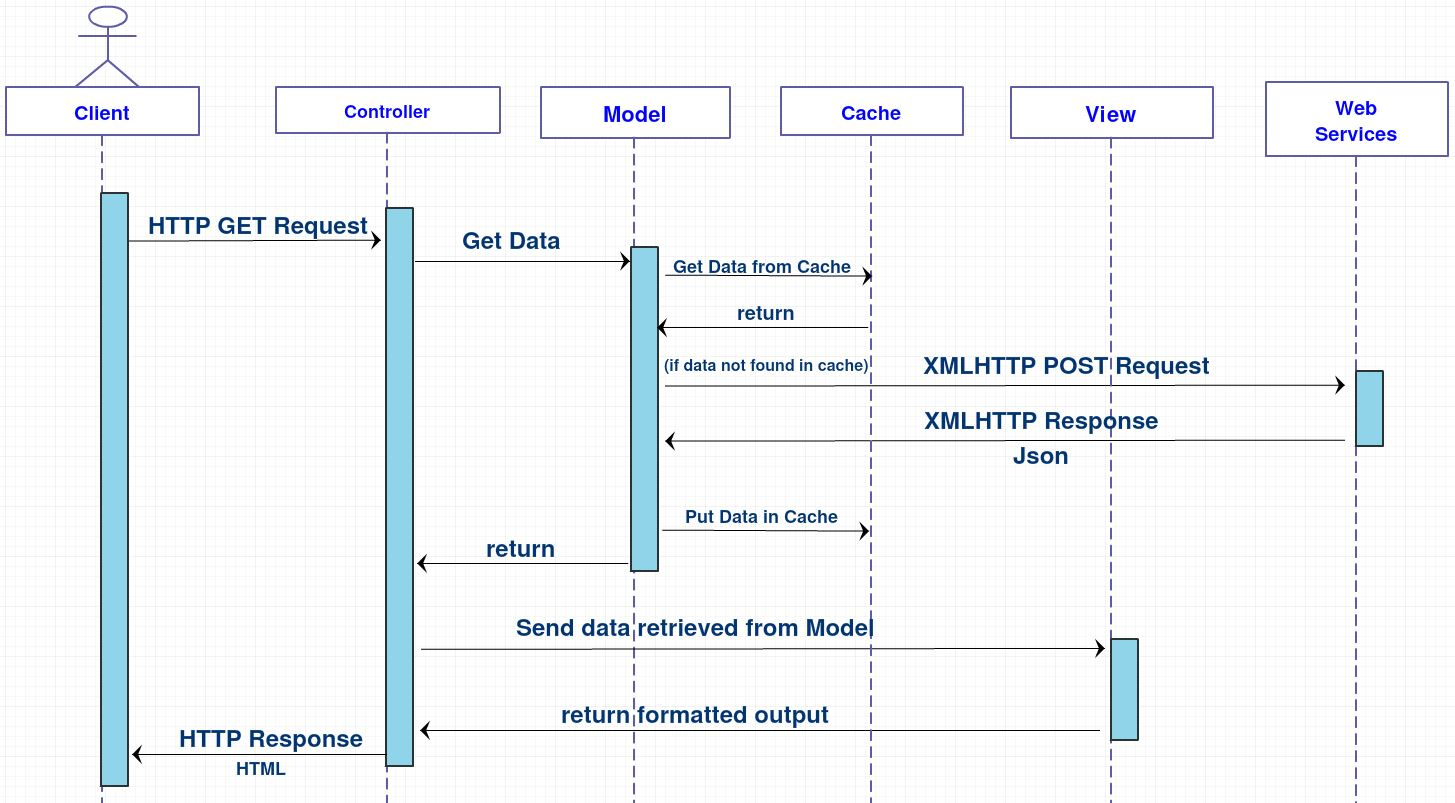
\includegraphics[height=5cm,width=7cm]{images/HTTPRequestSequenceDiagram}
		\caption{HTTP Request Sequence diagram}
		\label{HTTPRequest}
	\end{subfigure}
	\begin{subfigure}{.5\textwidth}
		\centering
		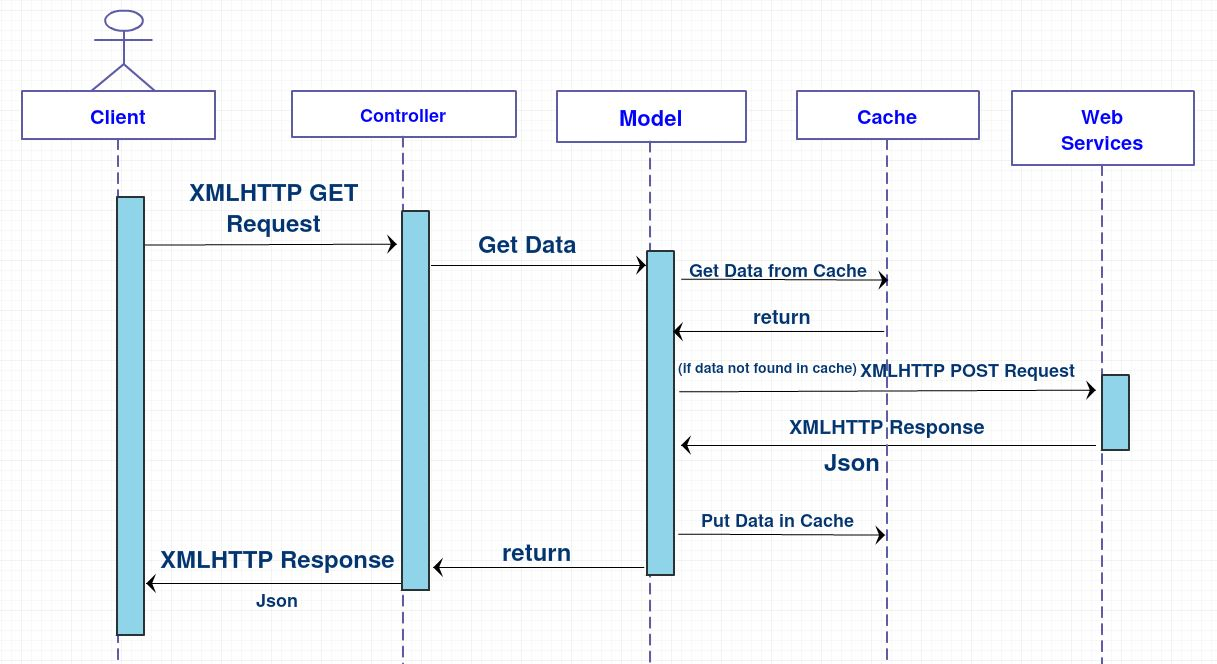
\includegraphics[height=5cm,width=7cm]{images/XMLHTTPRequestSequenceDiagram}
		\caption{XMLHTTP Request Sequence diagram}
		\label{XMLHTTPRequest}
	\end{subfigure}
	\caption{Components communication}
\end{figure}

\clearpage

\section{Security}
  

\section{Choice of technology}

say why we are using the browser and not native
\subsection{Web Application Framework}

\subsubsection{Play Framework}
\paragraph{}
Play Framework 2 is is an open source web application framework, written in Scala and Java, which follows the model–view–controller (mvc) architectural pattern. 
\\ \textbf{Pros}:
\begin{itemize}

\item It dramatically improves the productivity of a developer compared to other Java based web frameworks like Jersey or Spring MVC. The server not always has to be restarted in order to see the changes. \textit{Hot reload} is available for all Java classes, templates and configurations allows for much rapid development. This is available in many dynamic languages, but it is not provided in any other Java framework.

\item Play 2 is open source. If required, everything can be seen how it works. It has a relatively large community, represented by questions on StackOverflow and developers that contribute with developing plug-ins.

\item Java: type safe language. Also JVM performs great and can scale to support many developers and users. Furthermore, Java by itself has a large community and 
wide variety of IDEs\footnote{Integrated Development Environment} and available libraries.
	
\end{itemize}
\textbf{Cons}:
\begin{itemize}
\item Play 2 is relatively new framework so the community is not as big compared to other Java frameworks. 

\item The framework is immature. Not all bugs have been fixed and good practises are still no clearly defined. 

\item Java does not provide features like closures to keep asynchronous code clean. Play is build on top of asynchronous input and output. There are ways to go around this but the application will end up with lots of inner anonymous classes, which will reduce the maintainability and readability of the code.

\item Java does not support Json natively so a third-party library must be used. This, together with its strict types, will lead to big overheads when parsing Json, which 
is going to be the main source of data for this project.  
\end{itemize}

\subsubsection{Django}
\paragraph{}
Django is free and open source web application framework, written in Python. Its main focus is helping developers to write code, without the need to reinvent the wheel.
\\ \textbf{Pros}:
\begin{itemize}
	\item Django follows the DRY principle: Do not Repeat Yourself. The frameworks is designed so that developers can get the most out of little piece of code. In addition, this automatically leads to less hours spent in developing and lower chance of introducing bugs.
	\item Good documentation. Django provides sufficient documentation for every release with plenty of code examples. Furthermore, if something is not documented, the code is publicly available on GitHub so 
	it can be direclty inspected from there or from an IDE like PyCharm. 
	\item Django provides build-in Admin panel, that is generated automatically for each project. It allows users to manipulate and control users or database objects, specific to the application.
	\item Django is scalable as it is design on a component based architecture. All the components are decoupled and does not depend on each other so they can be easily unplugged and replaces. Likewise, new components can be simple to introduced. 
	\item Provides a set of tools that can be useful when writing tests. Tests can be perform not only on the Models and the Controllers, but also on the Views without a third-party library. It provides a build-in request factory, which uses URL resolution to trigger the views. 
\end{itemize}

\textbf{Cons}:
\begin{itemize}
	\item Django is using Python, that is an interpreted language, and it is ofthen slower than compiled languages.  
	\item If the application is using a database, long queries that make use of multiple JOINs or UNIONs can be quite hard to implement.  
\end{itemize}
\subsubsection{Laravel}
\paragraph{}
Laravel is a free, open-source PHP web framework, intended for the development of web applications following the model–view–controller (MVC) architectural pattern.
\\ \textbf{Pros}:
\begin{itemize}
	\item Composer - packaging system for PHP and is used for dependency management. Laravel is designed using a component based architecture and the whole framework is available as individual Composer packages. 
	\item Blade is the Laravel's template engine that is ligthweight and provides clean synstax for views. It supports template inheritance that reduces the duplication of code and reusability of specific template components. 
	\item Resourceful controllers. 
\end{itemize}
	
	
\textbf{Cons}:
\begin{itemize}
	\item test
\end{itemize}

\subsection{Javascript}

\subsection{CSS}

\subsection{Chart}

\subsection{Map}

\subsection{Javascript Library}

\subsection{CSS Framework}

\subsection{Chart}

\subsection{Map}



\chapter{Implementation}

\section{Model}

\section{View}

\section{Controller}

\section{Challenges}

\chapter{Evaluation}

\section{Product evaluation}

\subsection{Initial phase}

\subsection{Final phase}

\section{Testing}

\chapter{Future work}

%%%%%%%%%%%%%%%%
%              %
%  APPENDICES  %
%              %
%%%%%%%%%%%%%%%%
\begin{appendices}

\chapter{Running the Programs}
An example of running from the command line is as follows:
\begin{verbatim}
      > java MaxClique BBMC1 brock200_1.clq 14400
\end{verbatim}
This will apply $BBMC$ with $style = 1$ to the first brock200 DIMACS instance allowing 14400 seconds of cpu time.

\chapter{Generating Random Graphs}
\label{sec:randomGraph}
We generate Erd\'{o}s-R\"{e}nyi random graphs $G(n,p)$ where $n$ is the number of vertices and
each edge is included in the graph with probability $p$ independent from every other edge. It produces
a random graph in DIMACS format with vertices numbered 1 to $n$ inclusive. It can be run from the command line as follows to produce 
a clq file
\begin{verbatim}
      > java RandomGraph 100 0.9 > 100-90-00.clq
\end{verbatim}
\end{appendices}

%%%%%%%%%%%%%%%%%%%%
%   BIBLIOGRAPHY   %
%%%%%%%%%%%%%%%%%%%%

\bibliographystyle{plain}
\bibliography{bib}

\end{document}
